% 原书 p.147–p.153（PDF p.155–p.161）
\section{混沌的哈密顿动力学（Chaotic Hamiltonian Dynamics）}

% >>> p155
本节中，我们工作在辛非球面的（symplectically aspherical）流形 $(M,\omega)$ 上，即
满足 (5.16) 中条件的流形。5.4 节的构造对任意非退化哈密顿函数
$H\colon[0,1]\times M\to\R$ 与通有的近复结构 $J$，给出一个良定义的哈密顿 Floer
同调 $\mathrm{HF}_*(M,\omega,H,J)$。

把 $\mathrm{HF}_*(M,\omega,H,J)$ 升级为一个持续 $\Z_2$-模（见定义 5.2.1），记作
\[
  \mathbb{V}_H=\bigl((\{\mathbb{V}_{H,t}\}_{t\in\R}),
  (\{\iota_{s,t}\colon\mathbb{V}_{H,s}\to\mathbb{V}_{H,t}\}_{s\le t\in\R})\bigr),
\]
其中
\begin{equation}\tag{6.2}
  \mathbb{V}_{H,t}:=\mathrm{HF}_*(\{\mathcal{A}_H<t\};\Z_2)
\end{equation}
是那些在 (5.17) 所定义的作用量 $\mathcal{A}_H$ 下作用量小于 $t$ 的闭哈密顿轨道所
生成的同调群。这与例 5.2.2 的做法完全一致，因为 $\mathrm{HF}_*(M,\omega,H,J)$ 可以
看作无穷维 Morse 同调。同样在例 5.2.2 中，我们留下了一个问题：当我们改变 Morse
函数时，相应的持续模如何变化？这里出现了同样的问题。

\begin{keytakeaways}
\begin{itemize}
  \item 几何图像：对哈密顿函数作「过滤」，把哈密顿 Floer 同调连同其作用量过滤
        一起打包成一个持续模 $\mathbb{V}_H$；它的条形码（barcode）是动力学的
        「指纹」。
  \item 数学工具：条形码之间的瓶颈距离 $d_{\mathrm{bottleneck}}$ 把两个持续模的
        比较转化为 $\R^2$ 中两组点的定量比较；$\delta$-匹配是其定义的核心。
  \item 关键定理：Polterovich--Shelukhin 定理（定理 6.2.1）给出
        $d_{\mathrm{bottleneck}}\bigl(\mathbb{B}(\mathbb{V}_\varphi),
        \mathbb{B}(\mathbb{V}_\psi)\bigr)\le d_{\mathrm{Hofer}}(\varphi,\psi)$，
        把 Hofer 几何与代数（条形码）联系起来。
  \item 本节结论：由此可定义 $K$-Hofer 混沌（定义 6.2.2），并证明某些闭辛流形上
        Hofer 度量空间的直径无限（定理 6.2.2、注 6.2.4）。
\end{itemize}
\end{keytakeaways}

\begin{wque}{6.2.1}
  当哈密顿函数 $H$ 变为 $G$ 时，$\mathbb{V}_H$ 与 $\mathbb{V}_G$ 之间有怎样的
  关系？
\end{wque}

回忆定理 5.2.1：一个持续 $\Z_2$-模与其条形码一一对应。对给定的哈密顿函数
$H\colon[0,1]\times M\to\R$，记 $\mathbb{B}(\mathbb{V}_H)$ 为如上定义的持续
$\Z_2$-模 $\mathbb{V}_H$ 的条形码。我们将在条形码的层面上比较两个这样的持续
$\Z_2$-模。为此，需要引入下述关键概念。

\begin{wrem}{6.2.1}
  为消除区间 $I\subset\R$ 的端点开、闭带来的歧义（它源自持续模的各种半连续性），
  在下文中，条形码中的所有区间或形如 $(a,b]$（左开右闭），或形如 $(a,\infty)$
  （左开）。
\end{wrem}

\begin{wdefn}{6.2.1（[55] 第 3.1 节中的定义）}
  对任意两个条形码 $\mathbb{B}_1$ 与 $\mathbb{B}_2$ 以及给定的 $\delta>0$，
  $\mathbb{B}_1$ 与 $\mathbb{B}_2$ 之间的一个 $\delta$-\textbf{匹配}由以下数据构成：
  \begin{enumerate}[label=(\roman*)]
    \item 子集 $(\mathbb{B}_1)_{\mathrm{short}}\subset\mathbb{B}_1$ 与
          $(\mathbb{B}_2)_{\mathrm{short}}\subset\mathbb{B}_2$，它们由（部分而非
          全部的）满足 $|b-a|\le 2\delta$ 的区间 $(a,b]$ 组成，并且
          \[
            \#\bigl(\mathbb{B}_1\setminus(\mathbb{B}_1)_{\mathrm{short}}\bigr)
            =\#\bigl(\mathbb{B}_2\setminus(\mathbb{B}_2)_{\mathrm{short}}\bigr);
          \]
    \item 一个双射
          $\sigma\colon\mathbb{B}_1\setminus(\mathbb{B}_1)_{\mathrm{short}}
          \to\mathbb{B}_2\setminus(\mathbb{B}_2)_{\mathrm{short}}$，满足：若
          $(c,d]=\sigma\bigl((a,b]\bigr)$，则 $|a-c|\le\delta$ 且
          $|b-d|\le\delta$；若 $(c,\infty)=\sigma\bigl((a,\infty)\bigr)$，则
          $|a-c|\le\delta$。
  \end{enumerate}
  于是，定义 $\mathbb{B}_1$ 与 $\mathbb{B}_2$ 之间的\textbf{瓶颈距离}为
  \[
    d_{\mathrm{bottleneck}}(\mathbb{B}_1,\mathbb{B}_2)
    :=\inf\{\delta\ge 0\mid
    \text{存在 }\mathbb{B}_1\text{ 与 }\mathbb{B}_2\text{ 之间的一个 }
    \delta\text{-匹配}\}.
  \]
\end{wdefn}

% [Tutor Note: 易错预警——定义 6.2.1 中两处细节极易抄错：(1)「短区间」的条件是
% $|b-a|\le 2\delta$（长度不超过 $2\delta$，而非 $\delta$）；(2) 匹配只要求
% \emph{补集} $\mathbb{B}_i\setminus(\mathbb{B}_i)_{\mathrm{short}}$ 之间建立双射，
% 短区间本身被允许「配对失败」。端点的容差恰为 $\delta$：左端点误差
% $\le\delta$、右端点误差 $\le\delta$，故一个区间被「整体移动」$\delta$ 是允许的。
% 又因区间约定为左开右闭 $(a,b]$，$\infty$-长区间的右端点不参与匹配。]

\begin{wrem}{6.2.2}
  如定义 6.2.1 的 (i) 那样选取 $(\mathbb{B}_*)_{\mathrm{short}}$，其主要理由是
  保证 $\mathbb{B}_*$（$*=1,2$）中的补集具有相同的基数（从而定义 6.2.1 的 (ii)
  中的双射才有意义）。一个等价的替代做法是：不删去某些「短」区间，而向
  $\mathbb{B}_*$ 中加入若干形如 $(a,a]$ 的区间（注意其长度为 $0$），使得所得的
  扩充条形码具有相同的基数。
\end{wrem}

定义 6.2.1 的一个动因是：对 $\R^2$ 中两族点给出定量的比较，其中我们把条形码中的
一个区间 $(a,b]$ 等同于 $\R^2$ 中的点 $(a,b)$（见图 6.3）。严格说来，被等同的点
$(a,b)$ 应落在 $\R^2$ 的上半区域，即满足 $b\ge a$ 的区域。

% >>> p156
下述例子说明，瓶颈距离 $d_{\mathrm{bottleneck}}$ 是相当容易计算的。

\begin{wexam}{6.2.1}
  设 $\mathbb{B}_1=\{(0,2],(2,\infty)\}$，$\mathbb{B}_2=\{(3,\infty)\}$。可以取
  $(\mathbb{B}_1)_{\mathrm{short}}=\{(0,2]\}$ 与
  $(\mathbb{B}_2)_{\mathrm{short}}=\varnothing$，然后构造双射
  $\sigma\colon(2,+\infty)\to(3,+\infty)$。取 $\delta=1$，

% >>> p157
显然 $\mathbb{B}_1$ 与 $\mathbb{B}_2$ 之间存在一个 $1$-匹配。事实上，$1$ 就是最优
标量，这意味着 $d_{\mathrm{bottleneck}}(\mathbb{B}_1,\mathbb{B}_2)=1$。\hfill$//$
\end{wexam}

\begin{figure}[htbp]
  \centering
  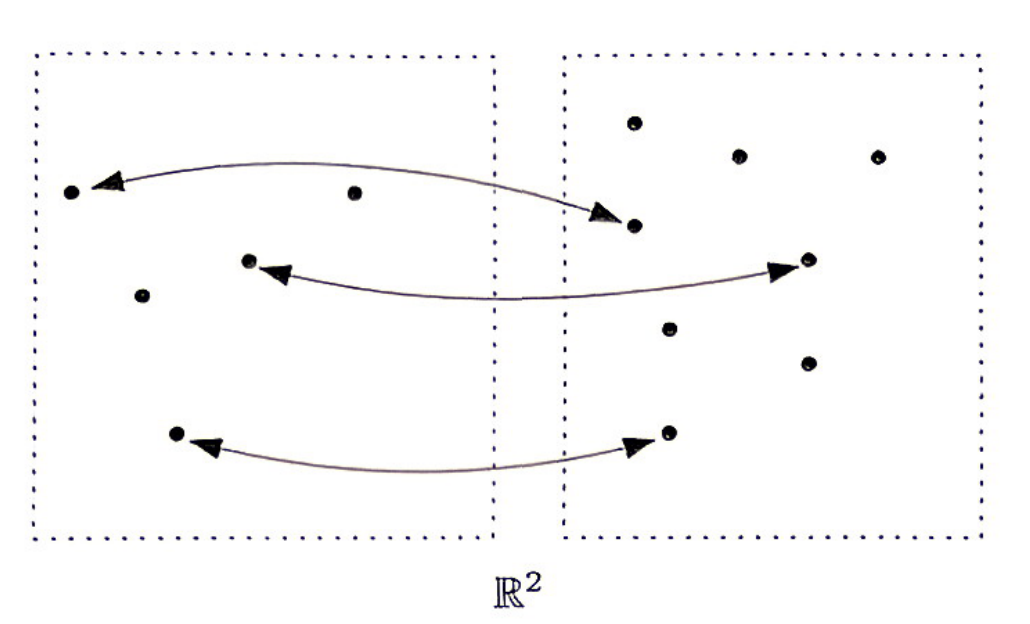
\includegraphics[width=0.62\linewidth]{figures/fig_p157_1.png}
  \caption*{图 6.3\quad $\R^2$ 中点的匹配（原书 p.149, Figure 6.3；PDF p.157）}
\end{figure}

\begin{wexam}{6.2.2}
  注意到：为得到关于 $d_{\mathrm{bottleneck}}$ 的最优匹配，一个 $\infty$-长区间
  必须与一个 $\infty$-长区间相匹配。因此，若 $\mathbb{B}_1$ 中 $\infty$-长区间的
  个数不等于 $\mathbb{B}_2$ 中 $\infty$-长区间的个数，则
  $d_{\mathrm{bottleneck}}(\mathbb{B}_1,\mathbb{B}_2)=+\infty$。还可验证：
  $d_{\mathrm{bottleneck}}(\mathbb{B}_1,\mathbb{B}_2)=0$ 当且仅当
  $\mathbb{B}_1=\mathbb{B}_2$。\hfill$//$
\end{wexam}

下述练习说明：即使只有条形码的部分信息，也能给出 $d_{\mathrm{bottleneck}}$ 的
有效估计。

\begin{wexer}{6.2.1（Lemma 5.1 in [211]）}
  设 $\mathbb{B}_1,\mathbb{B}_2$ 是两个条形码。设 $a_1\ge\cdots\ge a_n$ 为
  $\mathbb{B}_1$ 中区间的前 $n$ 个最小的左端点，相应的区间为
  $(a_1,c_{a_1}],\cdots,(a_n,c_{a_n}]$，其中 $c_{a_i}$ 可以是 $+\infty$。类似地，
  设 $b_1\ge\cdots\ge b_n$ 为 $\mathbb{B}_2$ 中区间的前 $n$ 个最小的左端点，
  相应的区间为 $(b_1,c_{b_1}],\cdots,(b_n,c_{b_n}]$。若
  $\min\{c_{a_1},\cdots,c_{a_n},c_{b_1},\cdots,c_{b_n}\}\ge\max\{a_1,b_1\}$，则
  \[
    \frac{1}{2}\max_{i=1,\cdots,n}|a_i-b_i|
    \le d_{\mathrm{bottleneck}}(\mathbb{B}_1,\mathbb{B}_2).
  \]
\end{wexer}

在回到问题 6.2.1 之前，先陈述下述事实：这是一个深刻的结果，表明（在某些情形下）
条形码的信息可以直接在哈密顿微分同胚的层面上提取出来，而不必先指定哈密顿函数。

\whead{事实}{6.2.1（cf.\ [200] 中的定理 1.2）}设 $(M,\omega)$ 是辛非球面辛流形
（即满足 (5.16) 中的条件）。则对规范化的 $H$，条形码 $\mathbb{B}(\mathbb{V}_H)$
在 $\Ham(M,\omega)$ 上是良定义的。换言之，对两个规范化哈密顿函数
$H,G\colon[0,1]\times M\to\R$，只要 $\varphi_H^1=\varphi_G^1\,(=\varphi)$，就有
$\mathbb{B}(\mathbb{V}_H)=\mathbb{B}(\mathbb{V}_G)$（因此，可以放心地把它记作
$\mathbb{B}(\mathbb{V}_\varphi)$）。

另一方面，下述事实给出了第一个（也是极为罕见的）例子：来自哈密顿动力学的条形码
$\mathbb{B}(\mathbb{V}_\varphi)$ 可以被显式地算出来。

% >>> p158
\whead{事实}{6.2.2（cf.\ [195] 中的定理 7.1）}设 $(M,\omega)$ 是辛非球面辛流形。
若 $\varphi=\varphi_H^1\in\Ham(M,\omega)$，其中 $H$ 是 $M$ 上 $C^2$-小的时间无关
规范化 Morse 函数，则
\begin{equation}\tag{6.3}
  \mathbb{B}(\mathbb{V}_\varphi)=\mathbb{B}(\mathbb{V}_H),
\end{equation}
其中 (6.3) 的右端是由过滤 Morse 同调群构造的持续 $\Z_2$-模 $\mathbb{V}_H$ 的条形码
（见例 5.2.2）。

下述例子是事实 6.2.2 的直接应用。

\begin{wexam}{6.2.3}
  设 $(M,\omega)$ 是闭辛非球面辛流形。则对 $M$ 上任意 $C^2$-小的时间无关规范化
  Morse 函数 $H$，存在点 $p\in\Crit(H)$ 使得 $\max_M H=H(p)>0$。于是事实 6.2.2
  蕴含 $\mathbb{B}(\mathbb{V}_\varphi)$ 包含一个区间 $(H(p),+\infty)$。\hfill$//$
\end{wexam}

现在我们可以用下述定理来回答问题 6.2.1，该定理把代数与动力学联系在了一起。

\begin{wthm}{6.2.1（Polterovich--Shelukhin [183]）}
  设 $(M,\omega)$ 是闭辛非球面辛流形。则对任意
  $\varphi,\psi\in\Ham(M,\omega)$，有
  \[
    d_{\mathrm{bottleneck}}\bigl(\mathbb{B}(\mathbb{V}_\varphi),
    \mathbb{B}(\mathbb{V}_\psi)\bigr)\le d_{\mathrm{Hofer}}(\varphi,\psi).
  \]
\end{wthm}

该定理的证明将推迟到第 7 章、在引入 Floer 延拓映射这一技术之后给出。该定理有两个
直接应用：其一是描述来自退化哈密顿系统的条形码；其二是在辛非球面情形下快速证明
Hofer 距离 $d_{\mathrm{Hofer}}$ 的非退化性（定理 6.1.1）。

% [Tutor Note: 含糊点拨——定理 6.2.1 是「条形码的稳定性定理」在辛情形下的对应物：
% 它断言瓶颈距离被 Hofer 距离控制，即 $\varphi\mapsto\mathbb{B}(\mathbb{V}_\varphi)$
% 是 $1$-Lipschitz 的。其证明（第 7 章）用 Floer 延拓映射把两条哈密顿同痕的
% 过滤链复形联系起来，本质上是「条形码稳定性」的代数论证。注意不等式的方向：
% 只知瓶颈距离 $\le$ Hofer 距离，反向一般不成立，故它只能给出动力学的下界估计。]

\begin{wexam}{6.2.4}
  考虑辛非球面辛流形 $(M,\omega)$ 上的哈密顿微分同胚
  $\varphi=\mathbf{1}$。尽管它完全退化（cf.\ 定义 5.4.1），我们仍可把它看作一列
  哈密顿微分同胚 $\{\varphi_{H_i}^1\}_{i\in\N}$ 的极限：只要求 $H_i$ 按
  $|H_i|_{C^0}\to 0$ 的意义趋于 $0$。特别地，
  $d_{\mathrm{Hofer}}(\varphi_{H_i}^1,\mathbf{1})\to 0$。于是定理 6.2.1 蕴含：
  在 $d_{\mathrm{bottleneck}}$ 之下，条形码
  $\mathbb{B}(\mathbb{V}_{\varphi_{H_i}^1})$ 收敛到以重数
  $\sum_i b_i(M;\Z_2)$ 计的区间 $(0,\infty)$ 之集。于是可以简单地定义
  \[
    \mathbb{B}(\mathbb{V}_{\mathbf{1}})
    :=\left\{(0,\infty)\;\middle|\;
    \text{以重数 }\sum_i b_i(M;\Z_2)\right\}.
  \]
  注意这个重数恰好就是总 Betti 数，这一点在经典 Morse 同调理论中也有体现
  （见练习 5.1.3 正下方的那一段）。\hfill$//$
\end{wexam}

\begin{wexam}{6.2.5（定理 6.1.1 在 $(M,\omega)$ 闭且辛非球面时的证明）}
  由命题 6.1.1，只需证明 Hofer 范数 $\|\cdot\|_{\mathrm{Hofer}}$ 不恒为零。
  事实上，取 $M$ 上 $C^2$-小的规范化 Morse 函数 $H$，便有
% >>> p159
  \begin{align*}
    \|\varphi\|_{\mathrm{Hofer}}
    &=d_{\mathrm{Hofer}}(\varphi,\mathbf{1})
    \ge d_{\mathrm{bottleneck}}\bigl(\mathbb{B}(\mathbb{V}_{\varphi_H^1}),
      \mathbb{B}(\mathbb{V}_{\mathbf{1}})\bigr)\\
    &=d_{\mathrm{bottleneck}}\bigl(\mathbb{B}(\mathbb{V}_H),
      \mathbb{B}(\mathbb{V}_{\mathbf{1}})\bigr)
    \ge\max_M H>0,
  \end{align*}
  其中第一个不等式来自定理 6.2.1，第二个等式来自例 6.2.3 中的 (6.3)，第二个
  不等式来自 $d_{\mathrm{bottleneck}}$ 的定义（特别是例 6.2.2 中关于
  $\infty$-长区间匹配的观察）。这就完成了证明。\hfill$//$
\end{wexam}

% [Tutor Note: 原文疑误——例 6.2.5 的证明中称「第二个等式来自例 6.2.3 中的 (6.3)」，
% 但 (6.3) 实际陈述于事实 6.2.2（例 6.2.3 只是其应用）。应改为「事实 6.2.2 中的
% (6.3)」。已记入 review_ch06.md。另注意最后一步 $\ge\max_M H>0$ 之所以成立，
% 是因为 $\mathbb{B}(\mathbb{V}_H)$ 含区间 $(H(p),\infty)$ 而
% $\mathbb{B}(\mathbb{V}_{\mathbf{1}})$ 含 $(0,\infty)$，二者作为 $\infty$-长区间
% 必须相配，端点差至少为 $H(p)$，再取 $p$ 使 $H$ 取最大值即得。]

\begin{wrem}{6.2.3}
  若给定的辛流形 $(M,\omega)$ 是闭的，则定理 6.2.1 也蕴含哈密顿 Floer 同调群
  $\mathrm{HF}_*$ 的不变性，即定理 5.4.1 中的第一个结论：
  $\mathrm{HF}_*(M,\omega,H,J)\cong\mathrm{HF}_*(M,\omega,H',J')$（作为
  $\Z_2$-模）。事实上，按定义有
  $d_{\mathrm{Hofer}}(\varphi_H^1,\varphi_{H'}^1)<\infty$，于是定理 6.2.1 蕴含
  $\mathbb{B}(\mathbb{V}_{\varphi_H^1})$ 与
  $\mathbb{B}(\mathbb{V}_{\varphi_{H'}^1})$ 具有相同个数的 $\infty$-长区间，
  而后者等于相应同调群的（总）秩。结合事实 6.2.2 中的 (6.3)，即得定理 5.4.1 的
  第二个结论。
\end{wrem}

借助 $d_{\mathrm{Hofer}}$，人们可以在哈密顿微分同胚的层面上定量地区分各种哈密顿
系统。如常所言，形式上最简单的动力系统来自时间无关（或称为\emph{自治}的）哈密顿
函数。为便于讨论，引入
\begin{equation}\tag{6.4}
  \Aut(M,\omega)=\left\{\varphi\in\Ham(M,\omega)\;\middle|\;
  \begin{array}{l}
    \varphi=\varphi_H^1\ \text{对某个}\\
    \text{时间无关的 } H
  \end{array}\right\}.
\end{equation}
一个把 $\Aut(M,\omega)$ 中元素与其他元素区分开来的巧妙观察是：$\Aut(M,\omega)$ 中
任何 $\varphi$ 都承认「方根」，即对任意素数 $p$，存在 $\psi\in\Aut(M,\omega)$
使得 $\psi^p=\varphi$。事实上，若 $\varphi=\varphi_H^1$，则哈密顿函数
$\frac{1}{p}H(x)$ 生成所需的 $\psi$。

% [Tutor Note: 术语/记号依据——$\Aut(M,\omega)$ 记「自治（autonomous）哈密顿
% 微分同胚」之集，它是 $\Ham(M,\omega)$ 中的子集而\emph{不是}子群：两个自治
% 微分同胚的复合一般不再是某个时间无关哈密顿函数的时间 1 映射。正因如此，
% 「$\Aut$ 中元素可开任意次方」才成为区别自治与非自治的动力学的判别特征，
% 并引出下面 $K$-Hofer 混沌的定义。]

为度量一个哈密顿系统「非自治」到什么程度，可以引入下述定义。

\begin{wdefn}{6.2.2}
  对给定的 $K>0$，若
  \begin{equation}\tag{6.5}
    d_{\mathrm{Hofer}}\bigl(\varphi,\Aut(M,\omega)\bigr)
    :=\inf_{\psi\in\Aut(M,\omega)}d_{\mathrm{Hofer}}(\varphi,\psi)\ge K,
  \end{equation}
  则称元素 $\varphi\in\Ham(M,\omega)$ 是 $K$-\textbf{Hofer 混沌}的，其中
  $\Aut(M,\omega)$ 是 (6.4) 中定义的 $\Ham(M,\omega)$ 的子集。
\end{wdefn}

由于混沌在我们这个世界中的普遍性，一个自然的问题是：是否总能找到一列哈密顿
微分同胚 $\{\varphi_i\}_{i\in\N}\subset\Ham(M,\omega)$，使得每个 $\varphi_i$ 对
某个 $K_i>0$ 是 $K_i$-Hofer 混沌的，且 $K_i\to\infty$（$i\to\infty$）？

% >>> p160
解决此问题的一条途径（受上面观察到的 $\Aut(M,\omega)$ 中元素的方根性质启发）是：
考察一般的 $\Ham(M,\omega)$ 中元素在多大程度上\emph{不}承认方根。下面介绍
[12] 中说明的一个策略，它最初来自 [157]。例如，取 $p=2$ 并考虑
\[
  \mathrm{Power}_2(M,\omega):=\{\varphi\in\Ham(M,\omega)\mid
  \varphi=\psi^2\ \text{对某个 }\psi\in\Ham(M,\omega)\}.
\]
于是 $\mathbb{V}_\varphi$ 上存在一个明显的 $\Z_2$-作用，具体由
\[
  x(t)\mapsto\psi\bigl(x(t)\bigr)
\]
给出。事实上，若 $x(1)\in\mathrm{Fix}(\varphi)$，则 $\psi(x(1))$ 满足
\[
  \varphi\bigl(\psi(x(1))\bigr)=\psi^3(x(1))
  =\psi\bigl(\varphi(x(1))\bigr)=\psi(x(1)),
\]
这表明 $\psi(x(t))$ 同样是哈密顿 Floer 同调群的生成元。

另一方面，用 $\psi$ 作「旋转」并不改变 (5.17) 中定义的辛作用量泛函
$\mathcal{A}_H$（因此相应的过滤同调群保持不变）。然而，关于这个 $\Z_2$-作用，
我们没有太多富有启发的话可说。让我们引入一个（源自 Milnor 的）技巧：若考虑
$\mathbb{V}_{\varphi^2}$（而非上面讨论的 $\mathbb{V}_\varphi$），则由同样的论证，
$\mathbb{V}_{\varphi^2}$ 上存在一个 $\Z_2$-作用，由
$x(t)\to\varphi(x(t))$ 给出。取该 $\Z_2$-作用的 $(-1)$-特征子空间；可以验证它是
一个良定义的持续 $\Z_2$-模，记作 $\mathbb{L}_{-1}(\varphi^2)$。仍在假设
$\varphi=\psi^2$ 之下，$\mathbb{V}_{\varphi^2}$ 上还有一个 $\Z_4$-作用，由
$x(t)\to\psi(x(t))$ 给出，记作 $P_\psi$。重要的是，限制到
$\mathbb{L}_{-1}(\varphi^2)$ 上时，有
\begin{equation}\tag{6.6}
  \bigl(P_\psi|_{\mathbb{L}_{-1}(\varphi^2)}\bigr)^2=-\mathbf{1}.
\end{equation}

作为形式上的比较，一个复结构 $\sqrt{-1}$ 满足 $(\sqrt{-1})^2=-\mathbf{1}$。
下述练习表明，条形码 $\mathbb{B}(\mathbb{L}_{-1}(\varphi^2))$ 中每个区间的重数
都是偶数。

\begin{wexer}{6.2.2}
  设 $\mathbb{V}$ 是一个持续模，配有持续态射
  $J\colon\mathbb{V}\to\mathbb{V}$（见练习 5.2.2），其中
  $J=\{J_t\colon\mathbb{V}_t\to\mathbb{V}_t\}_{t\in\R}$ 且
  $J_t^2=-\mathbf{1}_{\mathbb{V}_t}$。此外，对任意区间 $I\subset\R$，记
  \[
    m\bigl(I,\mathbb{B}(\mathbb{V})\bigr)
    =\#\{\mathbb{B}(\mathbb{V})\ \text{中包含 } I\ \text{的条}\}.
  \]
  证明：对任意 $I\subset\R$，数 $m(I,\mathbb{B}(\mathbb{V}))$ 总是偶数。
\end{wexer}

一般地，对任意素数 $p$ 与任意 $p$ 次单位根 $\zeta$（$\zeta\ne 1$），
$\mathbb{B}(\mathbb{L}_\zeta(\varphi^p))$ 中每个区间的重数都能被 $p$ 整除。这给出
$\varphi\in\Ham(M,\omega)$ 不属于 $\mathrm{Power}_p(M,\omega)$ 的一个障碍
（特别地，$\Aut(M,\omega)\subset\mathrm{Power}_p(M,\omega)$）。以此为基础，借助更
精细的论证，可以证明下述结果。

% >>> p161
\begin{wthm}{6.2.2（[183, 245]）}
  设 $(N,\omega_N)$ 是任意闭辛流形。则在乘积辛流形
  $\bigl(\Sigma_{g\ge 4}\times N,\pi_1^*\omega_{\mathrm{area}}
  +\pi_2^*\omega_N\bigr)$ 上，总存在一列哈密顿微分同胚
  $\{\varphi_i\}_{i\in\N}$，使得每个 $\varphi_i$ 是 $K_i$-Hofer 混沌的（对每个
  $i$），且 $K_i\to\infty$。
\end{wthm}

除上述 $\Aut(M,\omega)$ 中元素的 $p$-整除性之外，作为定理 6.2.2 证明中的另一个
关键步骤（为得到下界 $K_i$），定理 6.2.1 有助于把这个 Hofer 几何问题转化为条形码
上的组合问题——至少对辛非球面的 $(N,\omega_N)$ 是如此。对更一般的
$(N,\omega_N)$，我们需要更强的机器，把（过滤的）哈密顿 Floer 链复形转化为条形码
（见 [232]）。

\begin{wrem}{6.2.4}
  定理 6.2.2 特别地蕴含：度量空间
  $\bigl(\Ham(\Sigma_{g\ge 4}\times N,\pi_1^*\omega_{\mathrm{area}}
  +\pi_2^*\omega_N),d_{\mathrm{Hofer}}\bigr)$ 的直径是无限的。事实上，辛几何中的
  一个著名猜想断言：任意闭辛流形的 Hofer 直径总是无限的。尽管该猜想已在许多情形下
  得到证实，但一般而言至今仍未解决（见 [141, 179, 200, 78, 151]）。
\end{wrem}

% [Tutor Note: 含糊点拨——注意定理 6.2.2 的论断是对\emph{乘积}流形
% $\Sigma_{g\ge4}\times N$ 而言的：这里必须取亏格 $g\ge 4$ 的曲面以提供足够的
% 「代数自由度」（本质上是对 $\Sigma_g$ 的映射类群/条形码组合结构作文章），
% 而 $N$ 只起「补足维数」的作用。$K$-Hofer 混沌的构造性证明用到了
% $\mathrm{Power}_p$ 的 $p$-整除障碍（较初等的下界）与定理 6.2.1 的条形码组合
% 论证（较强的下界）两部分；注 6.2.4 又把结论升级为 Hofer 直径无限这一猜想性
% 陈述的已知情形。阅读时不要把「直径无限」误当作已对一切闭辛流形证明。]
